Machine-to-Machine (M2M) authentication adalah proses verifikasi yang digunakan untuk mengautentikasi perangkat atau mesin yang terhubung ke jaringan, seperti komputer, perangkat IoT, atau perangkat mobile. Proses ini memastikan bahwa hanya perangkat yang sah yang dapat terhubung ke jaringan dan mengakses data atau layanan yang tersedia seperti skema pada Gambar \ref*{fig:m2m}.

M2M authentication dapat menggunakan berbagai metode, seperti pengenalan suara, pengenalan wajah, pengenalan sidik jari, atau kombinasi dari metode tersebut. Dalam beberapa kasus, M2M authentication juga dapat menggunakan teknologi kriptografi, seperti enkripsi atau sertifikat digital, untuk memastikan keamanan komunikasi antar perangkat.

\begin{figure}
    \centering
    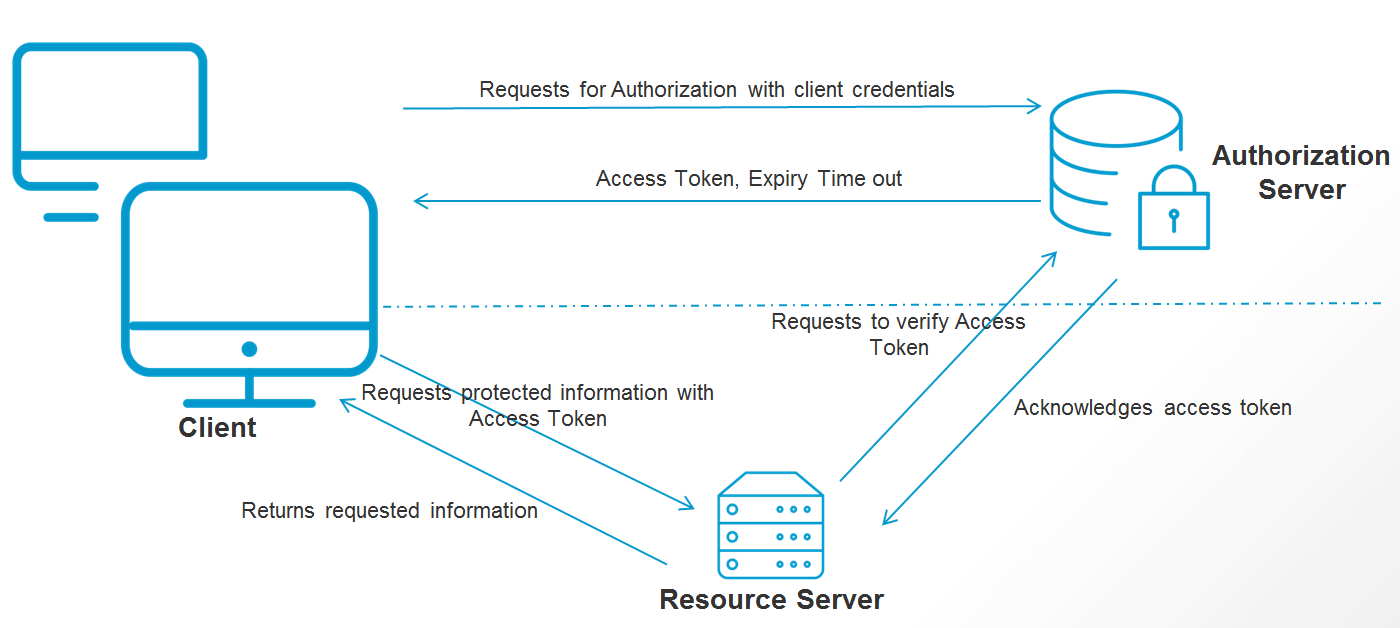
\includegraphics[width=0.8\textwidth]{BAB_TESIS/IMAGES/m2m_auth.png}
    \caption{Skema M2M Authentication}
    \label{fig:m2m}
\end{figure}